\documentclass{optica-article}
\usepackage{xcolor} 
\definecolor{darkred}{HTML}{BA1A1A}
\definecolor{extralightgray}{HTML}{F5F5F5}

\journal{opticajournal} % for journals or Optica Open

\articletype{Research Article}

\usepackage{lineno}
\usepackage{todonotes}
\usepackage{xcolor}
\usepackage{soul}
\providecommand{\tightlist}{%
  \setlength{\itemsep}{0pt}\setlength{\parskip}{0pt}}
\linenumbers % Turn off line numbering for Optica Open preprint submissions.

\begin{document}

\title{Data Recovery and Pulse Position Modulation with a Photon Number Resolving SNSPD}

\author{Author One,\authormark{1} Author Two,\authormark{2,*} and Author Three\authormark{2,3}}

\address{\authormark{1}Peer Review, Publications Department, Optica Publishing Group, 2010 Massachusetts Avenue NW, Washington, DC 20036, USA\\
\authormark{2}Publications Department, Optica Publishing Group, 2010 Massachusetts Avenue NW, Washington, DC 20036, USA\\
\authormark{3}Currently with the Department of Electronic Journals, Optica Publishing Group, 2010 Massachusetts Avenue NW, Washington, DC 20036, USA}

\email{\authormark{*}opex@optica.org} %% email address is required; see note below about the corresponding author designation

% use {asbstract*} to suppress the copyright line. Copyright information will be added in production

\begin{abstract*} 
Superconducting Nanowire Single Photon Detectors are a type of time-correlated photon detector with low jitter performance especially in the mid-infrared. They are useful for classical communication over high loss channels --such as across deep space-- and for quantum communication for which signals are restricted to the few-photon level. For classical communication, high photon information efficiency communication may be achieved with Pulse Position Modulation (PPM) whereby data is encoded in the arrival time of an optical pulse with respect to a clock. In the process of demonstrating PPM on a 20~Ghz clock, we study the effects of Photon Number Resolution (PNR) in new low-jitter types of SNSPDs. These PNR effects complicate fixed-threshold triggering of RF pulses from the SNSPD, and corrupt arrival time measurements if not properly managed. We demonstrate methods for simultaneous arrival time and photon number measurement which enables high clock rate PPM for space applications as well as high rate quantum communication and computing applications that benefit from photon number resolution.
\end{abstract*}

%%%%%%%%%%%%%%%%%%%%%%%%%%  body  %%%%%%%%%%%%%%%%%%%%%%%%%%
\hypertarget{introduction}{%
\section{Introduction}\label{introduction}}

Deep Space Optical Communication has been a growing field of study in recent years, as researchers look for ways to communicate with spacecraft that are far away from Earth. The main challenge in deep space optical communication is the high loss and distance that the link must traverse. This limits the communication from the spacecraft, as it is limited by the power available on the spacecraft. This means that the communication protocol is limited by the number of bits that can be sent per unit of energy on the spacecraft, also known as photon information efficiency or bits per photon.

In this article, we will focus on the use of Pulse Position Modulation (PPM) for space based optical communication. PPM involves sending a pulse in one of $2^M$ possible time slots. The transmission of each such pulse carries M bits of information based on when it arrives in a set of bins called a frame.

The Deep Space Optical Communicaiton (DSOC) project managed by the Jet Propulsion Laboratory (JPL) aims to demonstrate optical communication using PPM with the Psyche spacecraft from distances of \textbf{\hl{XX to XX}} Au.

For larger M, more data may be sent with a single optical pulse, thereby allowing a spacecrat to that is severely power limited to send more data over a high loss optical channel back to earth. This is quantified through the photon information efficiency $c_p = C/E$ where $C$ is the link capacity and $E$ is the photon cost per optical pulse

The existing deep space optical communication project uses M up to $2^8 = 256$, meaning that 8 bits of data may be carried in each optical pulse. M values as high as 19 have been demonstrated in the lab\cite{essiambre2023record}. However, the number of time bins needed per optical pulse scales exponentially with the number of bits transmitted per pulse. Therefore, for a given fixed clock rate and time bin duration, the PPM data rate decreases dramatically for higher M values.

We focus on demonstrating moderately large PIE, while also increasing the clock rate of the sytem by an order of magnitude relative to the DSOC platform (2\textasciitilde GHz). By operating at both higher clock rate and PIE than DSOC, this system exemplifies how future iterations of DSOC may send data more quickly but also over greater distances with the same power budget.

The increase in clock rate is made possible due to recent advancements in Niobium Nitride SNSPDs\textasciitilde{}\cite{Colangelo2023}. Low jitter performance is achieved by incorporating impedance matching tapers for efficient RF coupling, resulting in higher slew rate pulses, and by enabling RF pulse readout from both ends of the nanowire. The dual-ended readout allows for the cancellation of jitter caused by the variable location of photon arrival along the meander when the differential signals are recombined with a balun.
These detectors acheive jitter as low as 50 ps at the FW(1/100)M level, making them suitable for the demonstration of PPM with 50 ps slot widths and a 20 GHz clock.

\hypertarget{fig:intro}{%
\begin{figure}
\centering
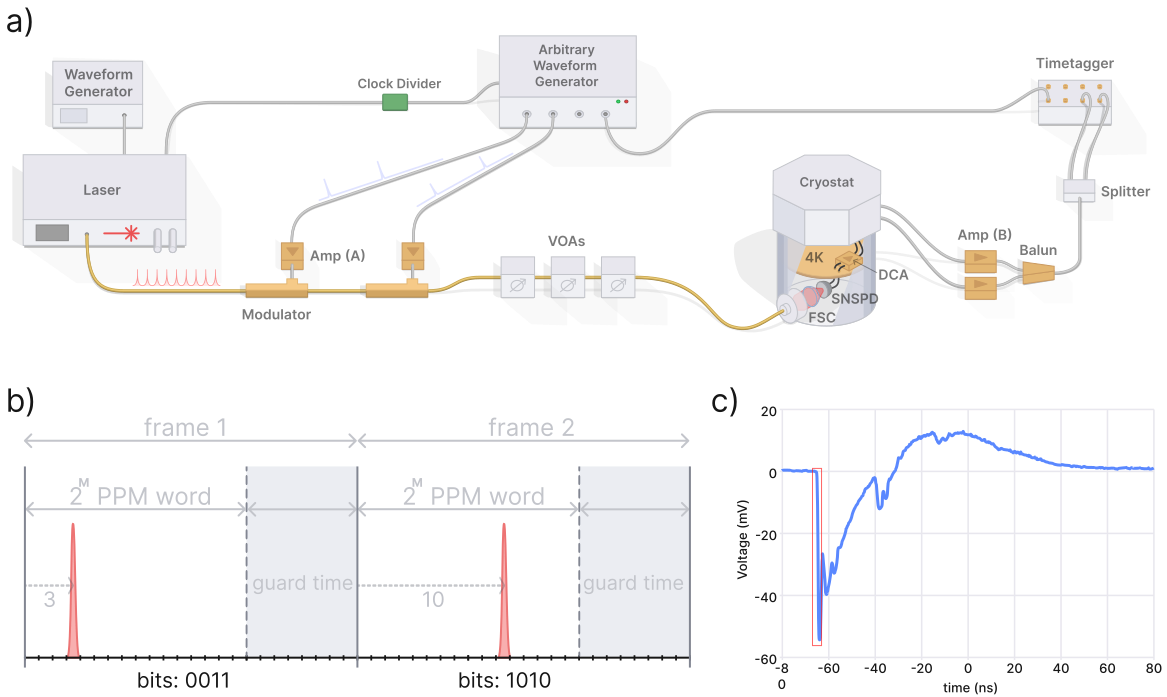
\includegraphics[width=1\textwidth]{./figs_03/fig_intro_2_light.pdf}
\caption[{PPM modulation and experiment setup}]{\textbf{PPM modulation and experiment setup} a) Diagram of the expiremental setup. WG: wave generator, CD: clock divider board, AWG: Arbitrary Waveform Generator, MLL: Mode Locked Laser (Pritel UAC), IM: Intensity Modulator, BC: Bias Controller, FSC: Free Space Coupling System, DCA: DC Coupled Cryo-amp b) How bits are transmitted in M=16 PPM modulation. An optical pulse is transmitted with a clock-referenced integer delay which encodes 4 bits of data. c) XXXXXXXX}
\label{fig:intro}
\end{figure}
}

However, the photon number number dependent response of these detectors is shown to affect the time-correlated measurements needed for high-rate PPM. This response, shown in Fig.~\ref{fig:waveform} is also known as photon number resolution (PNR) -- a property that is desirable in certain applications including quantum communication and quantum computing.
The SNSPD generates RF pulses with greater amplitude and slew rate when detecting optical pulses with multiple photons. Photon number effects manifest in this lower jitter variety of SNSPD due to the more efficient coupling of the nanowire to the readout circuit through the impedance matching tapers. It is likely that these effects will be present in other new SNSPD types engineered for low jitter, whether the PNR resolution is desired or not.

As the PNR response affects the timing of fixed threashold timetaggs at any trigger level, it has a significant effect of the timing measurements used for the PPM demonstration. Any other applications illumnate these detectors with optical pulses of non-vanishing mean photon numbers will have to content with these effects as well. For this reason, we study the PNR response in detail and present two methods for managing it. We show how the photon number information can be deconvolved from the arrival time information, and how both de-correlated degrees of freedom can be measured simultaneously. This is applicable to certain types of high-rate quantum communication and computing systems.

\hypertarget{fig:waveform}{%
\begin{figure}
\centering
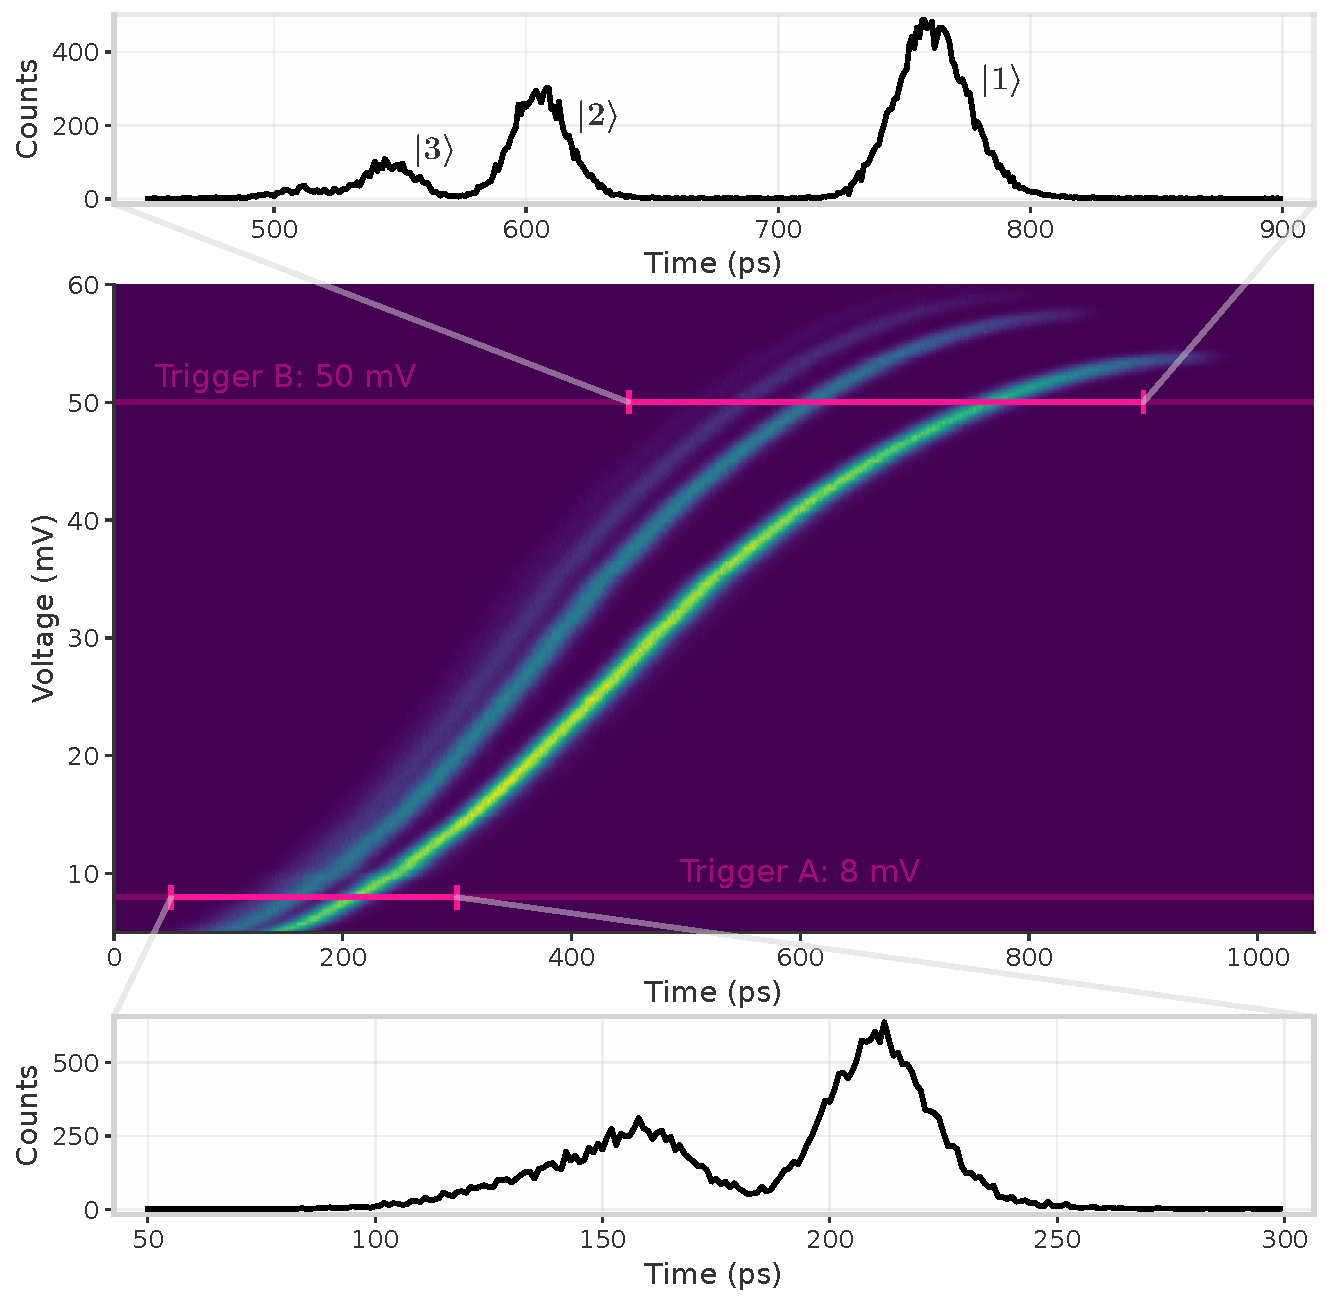
\includegraphics[width=0.8\textwidth]{./figs_03/waveform_light.pdf}
\caption[{PNR-sensitive Pulse Waveform}]{\textbf{PNR-sensitive Pulse Waveform} The rising edge of the differential SNSPD's RF pulses exibit variations in height, slew rate, and arrival time due to photon-number dependent dynamics. The slopes of the 1-photon and 2-photon pulses significantly differ, and as the photon number increases, the alterations to the pulse shape become progressively smaller. Trigger levels A (8~mV) and B (50~mV) were used to extract as much information about pulse slope and arrival time as possible}
\label{fig:waveform}
\end{figure}
}

\hypertarget{detector-figure-of-merit}{%
\section{Detector Figure of Merit}\label{detector-figure-of-merit}}

The work here highlights the application of low jitter single-photon detectors for optical communication, which is impactful for deep-space optical communication as well as classical communication in quantum networks. Although single-photon counting is well estanblished for deep-space optical communication\textasciitilde{}\cite{Laser lunar, DSOC} so far it has not been ulitized in quantum networks, mainly due to the use of SFP modules and DWDMs. However, with the eachievement of high data rates recently achieved with photon-counting classical communication, these approaches can now be seriously considered for quantum networks. The main driver is would be the deduction of optical power in neighbouring DWDM channels, which ultimately lowers the Raman scattered photons into the quantum channel \cite{EraerdsRaman}
\textbf{\hl{Calculate reduction in power from state of the art SFP modules}}

To access the applicability of different detectors, here we compare some of the recent near infrared detectors.

A useful figure of merit that includes all of the revelant detector metrics for photon timing was introduced by Bronzi and co-authors \cite{Bronzi2016}

$$FoM_T = \frac{\eta  (1 - P_{ap})\Phi_{-3 \text{dB}}}{J} \sqrt{\frac{A}{D}},$$

where $\eta$ is the single photon detection efficiency, $\Phi_{-3 \text{dB}}$ is the photon flux at which the system detection efficiency drops by 3\textasciitilde dB, $P_{ap}$ is the afterpulsing probability, $J$ is the detector jitter evaluated as the FWHM, $T_d$ is the deadtime, $A$ is the active area and $D$ is the dark count rate. Here we have defined the maximum photon flux as the 3\textasciitilde dB point, for ease of standardization.

In this work:

\begin{itemize}
\tightlist
\item
  Efficiency = 0.84
\item
  Afterpulsing = 0 %
\item
  Jitter = 15 ps
\item
  Deadtime = 30 ns \textbf{\hl{measure 3dB flux}}
\item
  Area = 330 $\mu m^2$
\item
  Dark count rate = 20~Hz
\end{itemize}

$FoM_T = 7.58 \times 10^{12}$ at 1550 nm.

The deadtime is calculated as the 1/MCR, which is the 3 dB point of the nominal efficiency. This is only a factor of 3.7 less than the state of the art visible Silicon SPADs (peak efficiency at 480~nm) \cite{Gramuglia2022}

In the future, the performance of the optical communication system could be improved by using, high count rate SNSPD arrays. Recently published high-count rate arrays have figures of merit of \textbf{\hl{$FoM_T$ for Peacoq and Resta2023 results}}. This would result in a proportinal increase in the data rate.
\textbf{\hl{$FoM_T$ for fastest InGaAs/InP gated detector}}
These devices are ideal for fiber-based optical communication. In free-space, the active area is especially important, whithout the use of an adaptive optics system.
\textbf{\hl{$FoM_T$ for DSOC array}}

\hypertarget{development-of-a-modulation-source}{%
\subsection{Development of a modulation source}\label{development-of-a-modulation-source}}

DSOC relies on modulation of a CW seed laser to generate the communication signal on the spacecraft. This signal is then amplified by an Erbium Doped Fiber Amplifier (EDFA) to increase its transmission power to Earth. As the EDFA amplifies the pre-generated pulses and uses most of the power of the spacecraft optical transmission system, power consumption scales with the number of optical pulses.

We produce our modulated singal by carving a series of mode locked laser pulses with lithium niobate modulators. This way, the jitter of the optical pulses themselves are not limited by the modulators or thew slew rate of the RF signal that drives them.

Therefore, we chose to carve pulses from a mode-locked laser. This approach allows for extremely short pulses in time, with the modulators responsible for sufficiently reducing any surrounding unwanted pulses. The temporal width of the modulator pulse response must be extremely short and able to modulate from `off' to `on' within a time frame of the order of the 50 ps bin width.

\hypertarget{methods}{%
\section{Methods}\label{methods}}

\hypertarget{slope-correction}{%
\subsection{Slope Correction}\label{slope-correction}}

\hypertarget{fig:slope-correction}{%
\begin{figure}
\centering
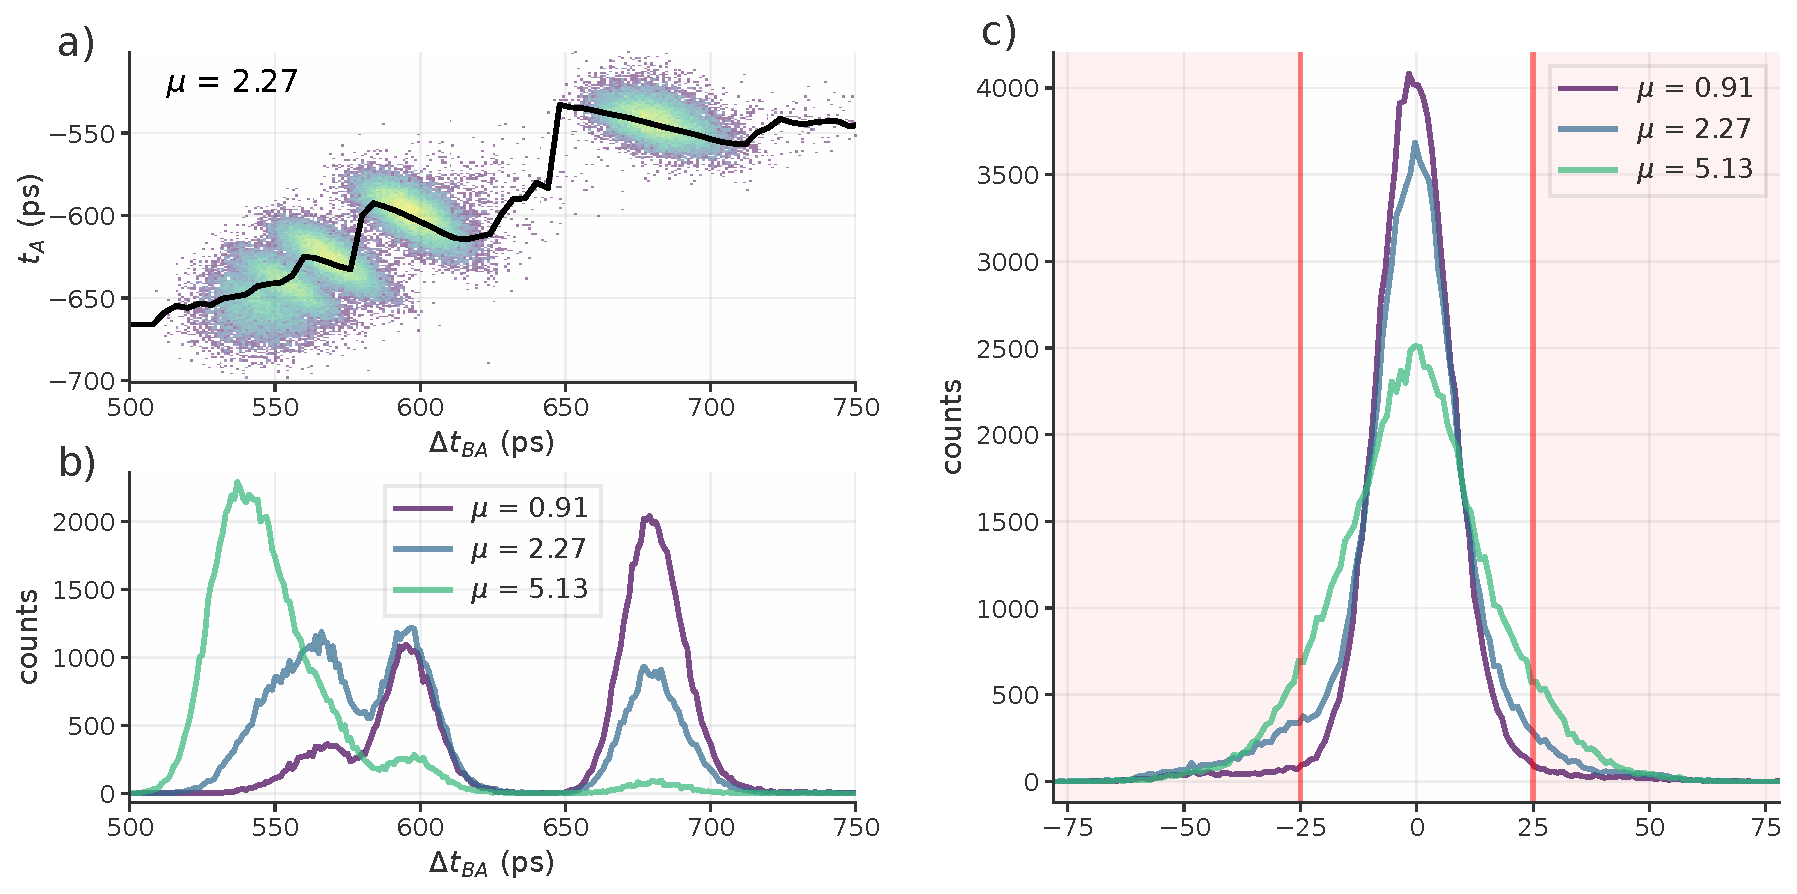
\includegraphics[width=0.75\textwidth]{./figs_03/slope_cancellation_light.pdf}
\caption[{PNR Slope Variation Analysis and Cancellation}]{\textbf{PNR Slope Variation Analysis and Cancellation} a) 2D histogram of RF pulse measurements. Through graphing slope $\Delta t_{BA}$ on the x-axis and arrival time $t_A$ on the y-axis, a series of groupings are visible that identify the discrete photon numbers detected.}
\label{fig:slope-correction}
\end{figure}
}

\hypertarget{cluster-analysis}{%
\subsection{Cluster Analysis}\label{cluster-analysis}}

\hypertarget{results}{%
\section{Results}\label{results}}

results here

\bibliography{references}



\end{document}